\documentclass[1p]{elsarticle_modified}
%\bibliographystyle{elsarticle-num}

%\usepackage[colorlinks]{hyperref}
%\usepackage{abbrmath_seonhwa} %\Abb, \Ascr, \Acal ,\Abf, \Afrak
\usepackage{amsfonts}
\usepackage{amssymb}
\usepackage{amsmath}
\usepackage{amsthm}
\usepackage{scalefnt}
\usepackage{amsbsy}
\usepackage{kotex}
\usepackage{caption}
\usepackage{subfig}
\usepackage{color}
\usepackage{graphicx}
\usepackage{xcolor} %% white, black, red, green, blue, cyan, magenta, yellow
\usepackage{float}
\usepackage{setspace}
\usepackage{hyperref}

\usepackage{tikz}
\usetikzlibrary{arrows}

\usepackage{multirow}
\usepackage{array} % fixed length table
\usepackage{hhline}

%%%%%%%%%%%%%%%%%%%%%
\makeatletter
\renewcommand*\env@matrix[1][\arraystretch]{%
	\edef\arraystretch{#1}%
	\hskip -\arraycolsep
	\let\@ifnextchar\new@ifnextchar
	\array{*\c@MaxMatrixCols c}}
\makeatother %https://tex.stackexchange.com/questions/14071/how-can-i-increase-the-line-spacing-in-a-matrix
%%%%%%%%%%%%%%%

\usepackage[normalem]{ulem}

\newcommand{\msout}[1]{\ifmmode\text{\sout{\ensuremath{#1}}}\else\sout{#1}\fi}
%SOURCE: \msout is \stkout macro in https://tex.stackexchange.com/questions/20609/strikeout-in-math-mode

\newcommand{\cancel}[1]{
	\ifmmode
	{\color{red}\msout{#1}}
	\else
	{\color{red}\sout{#1}}
	\fi
}

\newcommand{\add}[1]{
	{\color{blue}\uwave{#1}}
}

\newcommand{\replace}[2]{
	\ifmmode
	{\color{red}\msout{#1}}{\color{blue}\uwave{#2}}
	\else
	{\color{red}\sout{#1}}{\color{blue}\uwave{#2}}
	\fi
}

\newcommand{\Sol}{\mathcal{S}} %segment
\newcommand{\D}{D} %diagram
\newcommand{\A}{\mathcal{A}} %arc


%%%%%%%%%%%%%%%%%%%%%%%%%%%%%5 test

\def\sl{\operatorname{\textup{SL}}(2,\Cbb)}
\def\psl{\operatorname{\textup{PSL}}(2,\Cbb)}
\def\quan{\mkern 1mu \triangleright \mkern 1mu}

\theoremstyle{definition}
\newtheorem{thm}{Theorem}[section]
\newtheorem{prop}[thm]{Proposition}
\newtheorem{lem}[thm]{Lemma}
\newtheorem{ques}[thm]{Question}
\newtheorem{cor}[thm]{Corollary}
\newtheorem{defn}[thm]{Definition}
\newtheorem{exam}[thm]{Example}
\newtheorem{rmk}[thm]{Remark}
\newtheorem{alg}[thm]{Algorithm}

\newcommand{\I}{\sqrt{-1}}
\begin{document}

%\begin{frontmatter}
%
%\title{Boundary parabolic representations of knots up to 8 crossings}
%
%%% Group authors per affiliation:
%\author{Yunhi Cho} 
%\address{Department of Mathematics, University of Seoul, Seoul, Korea}
%\ead{yhcho@uos.ac.kr}
%
%
%\author{Seonhwa Kim} %\fnref{s_kim}}
%\address{Center for Geometry and Physics, Institute for Basic Science, Pohang, 37673, Korea}
%\ead{ryeona17@ibs.re.kr}
%
%\author{Hyuk Kim}
%\address{Department of Mathematical Sciences, Seoul National University, Seoul 08826, Korea}
%\ead{hyukkim@snu.ac.kr}
%
%\author{Seokbeom Yoon}
%\address{Department of Mathematical Sciences, Seoul National University, Seoul, 08826,  Korea}
%\ead{sbyoon15@snu.ac.kr}
%
%\begin{abstract}
%We find all boundary parabolic representation of knots up to 8 crossings.
%
%\end{abstract}
%\begin{keyword}
%    \MSC[2010] 57M25 
%\end{keyword}
%
%\end{frontmatter}

%\linenumbers
%\tableofcontents
%
\newcommand\colored[1]{\textcolor{white}{\rule[-0.35ex]{0.8em}{1.4ex}}\kern-0.8em\color{red} #1}%
%\newcommand\colored[1]{\textcolor{white}{ #1}\kern-2.17ex	\textcolor{white}{ #1}\kern-1.81ex	\textcolor{white}{ #1}\kern-2.15ex\color{red}#1	}

{\Large $\underline{12a_{0014}~(K12a_{0014})}$}

\setlength{\tabcolsep}{10pt}
\renewcommand{\arraystretch}{1.6}
\vspace{1cm}\begin{tabular}{m{100pt}>{\centering\arraybackslash}m{274pt}}
\multirow{5}{120pt}{
	\centering
	\includegraphics[width=112pt]{../../../GIT/diagram.site/Diagrams/png/815_12a_0014.png}\\
\ \ \ A knot diagram\footnotemark}&
\allowdisplaybreaks
\textbf{Linearized knot diagam} \\
\cline{2-2}
 &
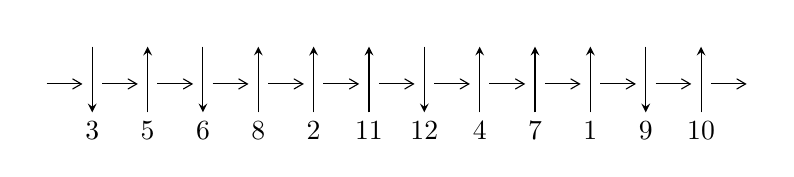
\begin{tikzpicture}[x=20pt, y=17pt]
	% nodes
	\node (C0) at (0, 0) {};
	\node (C1) at (1, 0) {};
	\node (C1U) at (1, +1) {};
	\node (C1D) at (1, -1) {3};

	\node (C2) at (2, 0) {};
	\node (C2U) at (2, +1) {};
	\node (C2D) at (2, -1) {5};

	\node (C3) at (3, 0) {};
	\node (C3U) at (3, +1) {};
	\node (C3D) at (3, -1) {6};

	\node (C4) at (4, 0) {};
	\node (C4U) at (4, +1) {};
	\node (C4D) at (4, -1) {8};

	\node (C5) at (5, 0) {};
	\node (C5U) at (5, +1) {};
	\node (C5D) at (5, -1) {2};

	\node (C6) at (6, 0) {};
	\node (C6U) at (6, +1) {};
	\node (C6D) at (6, -1) {11};

	\node (C7) at (7, 0) {};
	\node (C7U) at (7, +1) {};
	\node (C7D) at (7, -1) {12};

	\node (C8) at (8, 0) {};
	\node (C8U) at (8, +1) {};
	\node (C8D) at (8, -1) {4};

	\node (C9) at (9, 0) {};
	\node (C9U) at (9, +1) {};
	\node (C9D) at (9, -1) {7};

	\node (C10) at (10, 0) {};
	\node (C10U) at (10, +1) {};
	\node (C10D) at (10, -1) {1};

	\node (C11) at (11, 0) {};
	\node (C11U) at (11, +1) {};
	\node (C11D) at (11, -1) {9};

	\node (C12) at (12, 0) {};
	\node (C12U) at (12, +1) {};
	\node (C12D) at (12, -1) {10};
	\node (C13) at (13, 0) {};

	% arrows
	\draw[->,>={angle 60}]
	(C0) edge (C1) (C1) edge (C2) (C2) edge (C3) (C3) edge (C4) (C4) edge (C5) (C5) edge (C6) (C6) edge (C7) (C7) edge (C8) (C8) edge (C9) (C9) edge (C10) (C10) edge (C11) (C11) edge (C12) (C12) edge (C13) ;	\draw[->,>=stealth]
	(C1U) edge (C1D) (C2D) edge (C2U) (C3U) edge (C3D) (C4D) edge (C4U) (C5D) edge (C5U) (C6D) edge (C6U) (C7U) edge (C7D) (C8D) edge (C8U) (C9D) edge (C9U) (C10D) edge (C10U) (C11U) edge (C11D) (C12D) edge (C12U) ;
	\end{tikzpicture} \\
\hhline{~~} \\& 
\textbf{Solving Sequence} \\ \cline{2-2} 
 &
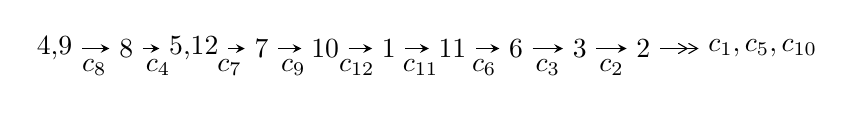
\begin{tikzpicture}[x=23pt, y=7pt]
	% node
	\node (A0) at (-1/8, 0) {4,9};
	\node (A1) at (1, 0) {8};
	\node (A2) at (33/16, 0) {5,12};
	\node (A3) at (25/8, 0) {7};
	\node (A4) at (33/8, 0) {10};
	\node (A5) at (41/8, 0) {1};
	\node (A6) at (49/8, 0) {11};
	\node (A7) at (57/8, 0) {6};
	\node (A8) at (65/8, 0) {3};
	\node (A9) at (73/8, 0) {2};
	\node (C1) at (1/2, -1) {$c_{8}$};
	\node (C2) at (3/2, -1) {$c_{4}$};
	\node (C3) at (21/8, -1) {$c_{7}$};
	\node (C4) at (29/8, -1) {$c_{9}$};
	\node (C5) at (37/8, -1) {$c_{12}$};
	\node (C6) at (45/8, -1) {$c_{11}$};
	\node (C7) at (53/8, -1) {$c_{6}$};
	\node (C8) at (61/8, -1) {$c_{3}$};
	\node (C9) at (69/8, -1) {$c_{2}$};
	\node (A10) at (11, 0) {$c_{1},c_{5},c_{10}$};

	% edge
	\draw[->,>=stealth]	
	(A0) edge (A1) (A1) edge (A2) (A2) edge (A3) (A3) edge (A4) (A4) edge (A5) (A5) edge (A6) (A6) edge (A7) (A7) edge (A8) (A8) edge (A9) ;
	\draw[->>,>={angle 60}]	
	(A9) edge (A10);
\end{tikzpicture} \\ 

\end{tabular} \\

\footnotetext{
The image of knot diagram is generated by the software ``\textbf{Draw programme}" developed by Andrew Bartholomew(\url{http://www.layer8.co.uk/maths/draw/index.htm\#Running-draw}), where we modified some parts for our purpose(\url{https://github.com/CATsTAILs/LinksPainter}).
}\phantom \\ \newline 
\centering \textbf{Ideals for irreducible components\footnotemark of $X_{\text{par}}$} 
 
\begin{align*}
I^u_{1}&=\langle 
-2.85861\times10^{554} u^{134}-1.62328\times10^{554} u^{133}+\cdots+7.59512\times10^{556} b+5.83950\times10^{556},\\
\phantom{I^u_{1}}&\phantom{= \langle  }6.60944\times10^{555} u^{134}+5.58826\times10^{555} u^{133}+\cdots+3.03805\times10^{557} a-5.01249\times10^{557},\\
\phantom{I^u_{1}}&\phantom{= \langle  }u^{135}+u^{134}+\cdots+5120 u+1024\rangle \\
\\
I^v_{1}&=\langle 
a,\;1728 v^9-4936 v^8+9872 v^7+12908 v^6-24680 v^5-34552 v^4+91527 v^3+4936 v^2+3335 b-613,\\
\phantom{I^v_{1}}&\phantom{= \langle  }v^{10}-3 v^9+6 v^8+7 v^7-16 v^6-19 v^5+58 v^4-2 v^3-7 v^2- v+1\rangle \\
\end{align*}
\raggedright * 2 irreducible components of $\dim_{\mathbb{C}}=0$, with total 145 representations.\\
\footnotetext{All coefficients of polynomials are rational numbers. But the coefficients are sometimes approximated in decimal forms when there is not enough margin.}
\newpage
\renewcommand{\arraystretch}{1}
\centering \section*{I. $I^u_{1}= \langle -2.86\times10^{554} u^{134}-1.62\times10^{554} u^{133}+\cdots+7.60\times10^{556} b+5.84\times10^{556},\;6.61\times10^{555} u^{134}+5.59\times10^{555} u^{133}+\cdots+3.04\times10^{557} a-5.01\times10^{557},\;u^{135}+u^{134}+\cdots+5120 u+1024 \rangle$}
\flushleft \textbf{(i) Arc colorings}\\
\begin{tabular}{m{7pt} m{180pt} m{7pt} m{180pt} }
\flushright $a_{4}=$&$\begin{pmatrix}0\\u\end{pmatrix}$ \\
\flushright $a_{9}=$&$\begin{pmatrix}1\\0\end{pmatrix}$ \\
\flushright $a_{8}=$&$\begin{pmatrix}1\\u^2\end{pmatrix}$ \\
\flushright $a_{5}=$&$\begin{pmatrix}u\\u^3+u\end{pmatrix}$ \\
\flushright $a_{12}=$&$\begin{pmatrix}-0.0217555 u^{134}-0.0183942 u^{133}+\cdots-118.348 u+1.64990\\0.00376375 u^{134}+0.00213726 u^{133}+\cdots+5.03100 u-0.768849\end{pmatrix}$ \\
\flushright $a_{7}=$&$\begin{pmatrix}0.0231345 u^{134}+0.0198385 u^{133}+\cdots+78.2695 u-13.5936\\-0.00174481 u^{134}+0.000798106 u^{133}+\cdots+7.06589 u+2.98825\end{pmatrix}$ \\
\flushright $a_{10}=$&$\begin{pmatrix}-0.0117679 u^{134}-0.0105468 u^{133}+\cdots-58.9017 u+4.02896\\-0.000139894 u^{134}-0.00437016 u^{133}+\cdots-30.6553 u-8.90982\end{pmatrix}$ \\
\flushright $a_{1}=$&$\begin{pmatrix}-0.00855818 u^{134}-0.00893424 u^{133}+\cdots-68.5627 u-7.86120\\-0.000139894 u^{134}-0.00437016 u^{133}+\cdots-30.6553 u-8.90982\end{pmatrix}$ \\
\flushright $a_{11}=$&$\begin{pmatrix}-0.0179918 u^{134}-0.0162570 u^{133}+\cdots-113.317 u+0.881056\\0.00376375 u^{134}+0.00213726 u^{133}+\cdots+5.03100 u-0.768849\end{pmatrix}$ \\
\flushright $a_{6}=$&$\begin{pmatrix}-0.00493334 u^{134}-0.00304908 u^{133}+\cdots-27.2183 u+1.43371\\0.00362484 u^{134}+0.00588516 u^{133}+\cdots+41.3444 u+9.29491\end{pmatrix}$ \\
\flushright $a_{3}=$&$\begin{pmatrix}-0.00927652 u^{134}-0.00766135 u^{133}+\cdots-11.8409 u+3.00848\\-0.00413661 u^{134}-0.00548717 u^{133}+\cdots-36.5774 u-8.33864\end{pmatrix}$ \\
\flushright $a_{2}=$&$\begin{pmatrix}-0.00806844 u^{134}-0.00630388 u^{133}+\cdots-11.2024 u+3.00445\\-0.00434251 u^{134}-0.00454724 u^{133}+\cdots-37.9408 u-8.49565\end{pmatrix}$\\&\end{tabular}
\flushleft \textbf{(ii) Obstruction class $= -1$}\\~\\
\flushleft \textbf{(iii) Cusp Shapes $= 0.0466570 u^{134}+0.0350645 u^{133}+\cdots+138.453 u-37.6705$}\\~\\
\newpage\renewcommand{\arraystretch}{1}
\flushleft \textbf{(iv) u-Polynomials at the component}\newline \\
\begin{tabular}{m{50pt}|m{274pt}}
Crossings & \hspace{64pt}u-Polynomials at each crossing \\
\hline $$\begin{aligned}c_{1}\end{aligned}$$&$\begin{aligned}
&u^{135}+64 u^{134}+\cdots+158 u-1
\end{aligned}$\\
\hline $$\begin{aligned}c_{2},c_{5}\end{aligned}$$&$\begin{aligned}
&u^{135}+6 u^{134}+\cdots-2 u-1
\end{aligned}$\\
\hline $$\begin{aligned}c_{3}\end{aligned}$$&$\begin{aligned}
&u^{135}-6 u^{134}+\cdots+18532724 u-1174793
\end{aligned}$\\
\hline $$\begin{aligned}c_{4},c_{8}\end{aligned}$$&$\begin{aligned}
&u^{135}- u^{134}+\cdots+5120 u-1024
\end{aligned}$\\
\hline $$\begin{aligned}c_{6}\end{aligned}$$&$\begin{aligned}
&u^{135}-3 u^{134}+\cdots+17948537 u-2522669
\end{aligned}$\\
\hline $$\begin{aligned}c_{7}\end{aligned}$$&$\begin{aligned}
&u^{135}+3 u^{134}+\cdots+12401 u-47809
\end{aligned}$\\
\hline $$\begin{aligned}c_{9}\end{aligned}$$&$\begin{aligned}
&u^{135}+9 u^{134}+\cdots+3 u+1
\end{aligned}$\\
\hline $$\begin{aligned}c_{10},c_{12}\end{aligned}$$&$\begin{aligned}
&u^{135}+3 u^{134}+\cdots+23 u-1
\end{aligned}$\\
\hline $$\begin{aligned}c_{11}\end{aligned}$$&$\begin{aligned}
&u^{135}-23 u^{134}+\cdots+3 u-1
\end{aligned}$\\
\hline
\end{tabular}\\~\\
\newpage\renewcommand{\arraystretch}{1}
\flushleft \textbf{(v) Riley Polynomials at the component}\newline \\
\begin{tabular}{m{50pt}|m{274pt}}
Crossings & \hspace{64pt}Riley Polynomials at each crossing \\
\hline $$\begin{aligned}c_{1}\end{aligned}$$&$\begin{aligned}
&y^{135}+20 y^{134}+\cdots+22410 y-1
\end{aligned}$\\
\hline $$\begin{aligned}c_{2},c_{5}\end{aligned}$$&$\begin{aligned}
&y^{135}+64 y^{134}+\cdots+158 y-1
\end{aligned}$\\
\hline $$\begin{aligned}c_{3}\end{aligned}$$&$\begin{aligned}
&y^{135}-24 y^{134}+\cdots+270394515667686 y-1380138592849
\end{aligned}$\\
\hline $$\begin{aligned}c_{4},c_{8}\end{aligned}$$&$\begin{aligned}
&y^{135}+55 y^{134}+\cdots-24117248 y-1048576
\end{aligned}$\\
\hline $$\begin{aligned}c_{6}\end{aligned}$$&$\begin{aligned}
&y^{135}+85 y^{134}+\cdots+285856654348325 y-6363858883561
\end{aligned}$\\
\hline $$\begin{aligned}c_{7}\end{aligned}$$&$\begin{aligned}
&y^{135}+149 y^{134}+\cdots-218902272299 y-2285700481
\end{aligned}$\\
\hline $$\begin{aligned}c_{9}\end{aligned}$$&$\begin{aligned}
&y^{135}-23 y^{134}+\cdots+9 y-1
\end{aligned}$\\
\hline $$\begin{aligned}c_{10},c_{12}\end{aligned}$$&$\begin{aligned}
&y^{135}-95 y^{134}+\cdots-23 y-1
\end{aligned}$\\
\hline $$\begin{aligned}c_{11}\end{aligned}$$&$\begin{aligned}
&y^{135}+9 y^{134}+\cdots-23 y-1
\end{aligned}$\\
\hline
\end{tabular}\\~\\
\newpage\flushleft \textbf{(vi) Complex Volumes and Cusp Shapes}
$$\begin{array}{c|c|c}  
\text{Solutions to }I^u_{1}& \I (\text{vol} + \sqrt{-1}CS) & \text{Cusp shape}\\
 \hline 
\begin{aligned}
u &= -0.433893 + 0.902869 I \\
a &= \phantom{-}0.425864 + 0.882091 I \\
b &= -0.003490 + 0.677446 I\end{aligned}
 & \phantom{-}0.69426 - 1.95174 I & \phantom{-0.000000 } 0 \\ \hline\begin{aligned}
u &= -0.433893 - 0.902869 I \\
a &= \phantom{-}0.425864 - 0.882091 I \\
b &= -0.003490 - 0.677446 I\end{aligned}
 & \phantom{-}0.69426 + 1.95174 I & \phantom{-0.000000 } 0 \\ \hline\begin{aligned}
u &= -0.088159 + 0.991363 I \\
a &= \phantom{-}0.526555 + 0.438584 I \\
b &= -0.02808 - 1.59756 I\end{aligned}
 & -1.95084 + 4.11866 I & \phantom{-0.000000 } 0 \\ \hline\begin{aligned}
u &= -0.088159 - 0.991363 I \\
a &= \phantom{-}0.526555 - 0.438584 I \\
b &= -0.02808 + 1.59756 I\end{aligned}
 & -1.95084 - 4.11866 I & \phantom{-0.000000 } 0 \\ \hline\begin{aligned}
u &= \phantom{-}0.631449 + 0.759674 I \\
a &= -0.118886 + 1.358980 I \\
b &= -1.16906 - 1.10258 I\end{aligned}
 & \phantom{-}4.93681 + 3.31408 I & \phantom{-0.000000 } 0 \\ \hline\begin{aligned}
u &= \phantom{-}0.631449 - 0.759674 I \\
a &= -0.118886 - 1.358980 I \\
b &= -1.16906 + 1.10258 I\end{aligned}
 & \phantom{-}4.93681 - 3.31408 I & \phantom{-0.000000 } 0 \\ \hline\begin{aligned}
u &= \phantom{-}0.502757 + 0.881596 I \\
a &= -2.43306 - 0.45379 I \\
b &= \phantom{-}0.96563 - 1.13597 I\end{aligned}
 & \phantom{-}0.83592 + 5.69951 I & \phantom{-0.000000 } 0 \\ \hline\begin{aligned}
u &= \phantom{-}0.502757 - 0.881596 I \\
a &= -2.43306 + 0.45379 I \\
b &= \phantom{-}0.96563 + 1.13597 I\end{aligned}
 & \phantom{-}0.83592 - 5.69951 I & \phantom{-0.000000 } 0 \\ \hline\begin{aligned}
u &= -0.815971 + 0.551004 I \\
a &= \phantom{-}1.58128 - 1.61392 I \\
b &= -1.03373 - 1.19051 I\end{aligned}
 & \phantom{-}3.37680 + 5.10317 I & \phantom{-0.000000 } 0 \\ \hline\begin{aligned}
u &= -0.815971 - 0.551004 I \\
a &= \phantom{-}1.58128 + 1.61392 I \\
b &= -1.03373 + 1.19051 I\end{aligned}
 & \phantom{-}3.37680 - 5.10317 I & \phantom{-0.000000 } 0\\
 \hline 
 \end{array}$$\newpage$$\begin{array}{c|c|c}  
\text{Solutions to }I^u_{1}& \I (\text{vol} + \sqrt{-1}CS) & \text{Cusp shape}\\
 \hline 
\begin{aligned}
u &= \phantom{-}0.723890 + 0.651860 I \\
a &= \phantom{-}1.72127 + 1.34248 I \\
b &= -1.20491 + 1.04638 I\end{aligned}
 & \phantom{-}4.99306 - 0.38975 I & \phantom{-0.000000 } 0 \\ \hline\begin{aligned}
u &= \phantom{-}0.723890 - 0.651860 I \\
a &= \phantom{-}1.72127 - 1.34248 I \\
b &= -1.20491 - 1.04638 I\end{aligned}
 & \phantom{-}4.99306 + 0.38975 I & \phantom{-0.000000 } 0 \\ \hline\begin{aligned}
u &= -0.286505 + 0.930576 I \\
a &= \phantom{-}1.90508 - 0.43378 I \\
b &= -1.67062 - 0.41030 I\end{aligned}
 & \phantom{-}0.509155 + 0.687850 I & \phantom{-0.000000 } 0 \\ \hline\begin{aligned}
u &= -0.286505 - 0.930576 I \\
a &= \phantom{-}1.90508 + 0.43378 I \\
b &= -1.67062 + 0.41030 I\end{aligned}
 & \phantom{-}0.509155 - 0.687850 I & \phantom{-0.000000 } 0 \\ \hline\begin{aligned}
u &= \phantom{-}0.820910 + 0.498296 I \\
a &= \phantom{-}0.438207 - 0.040079 I \\
b &= \phantom{-}0.89893 + 1.13522 I\end{aligned}
 & \phantom{-}1.03911 - 2.79672 I & \phantom{-0.000000 } 0 \\ \hline\begin{aligned}
u &= \phantom{-}0.820910 - 0.498296 I \\
a &= \phantom{-}0.438207 + 0.040079 I \\
b &= \phantom{-}0.89893 - 1.13522 I\end{aligned}
 & \phantom{-}1.03911 + 2.79672 I & \phantom{-0.000000 } 0 \\ \hline\begin{aligned}
u &= -0.941752 + 0.162453 I \\
a &= \phantom{-}0.409172 - 0.067675 I \\
b &= \phantom{-}0.981886 - 0.759449 I\end{aligned}
 & -2.45542 + 0.43451 I & \phantom{-0.000000 } 0 \\ \hline\begin{aligned}
u &= -0.941752 - 0.162453 I \\
a &= \phantom{-}0.409172 + 0.067675 I \\
b &= \phantom{-}0.981886 + 0.759449 I\end{aligned}
 & -2.45542 - 0.43451 I & \phantom{-0.000000 } 0 \\ \hline\begin{aligned}
u &= \phantom{-}0.893004 + 0.316819 I \\
a &= \phantom{-}0.456893 - 0.202993 I \\
b &= -0.299724 - 0.257774 I\end{aligned}
 & -0.44956 - 3.21138 I & \phantom{-0.000000 } 0 \\ \hline\begin{aligned}
u &= \phantom{-}0.893004 - 0.316819 I \\
a &= \phantom{-}0.456893 + 0.202993 I \\
b &= -0.299724 + 0.257774 I\end{aligned}
 & -0.44956 + 3.21138 I & \phantom{-0.000000 } 0\\
 \hline 
 \end{array}$$\newpage$$\begin{array}{c|c|c}  
\text{Solutions to }I^u_{1}& \I (\text{vol} + \sqrt{-1}CS) & \text{Cusp shape}\\
 \hline 
\begin{aligned}
u &= \phantom{-}0.590004 + 0.893147 I \\
a &= \phantom{-}1.68981 + 0.84924 I \\
b &= -1.59251 + 0.85847 I\end{aligned}
 & \phantom{-}4.52600 + 1.48756 I & \phantom{-0.000000 } 0 \\ \hline\begin{aligned}
u &= \phantom{-}0.590004 - 0.893147 I \\
a &= \phantom{-}1.68981 - 0.84924 I \\
b &= -1.59251 - 0.85847 I\end{aligned}
 & \phantom{-}4.52600 - 1.48756 I & \phantom{-0.000000 } 0 \\ \hline\begin{aligned}
u &= -0.445366 + 0.977234 I \\
a &= \phantom{-}0.452646 + 0.253352 I \\
b &= \phantom{-}0.44042 - 1.65879 I\end{aligned}
 & -0.79606 - 2.83608 I & \phantom{-0.000000 } 0 \\ \hline\begin{aligned}
u &= -0.445366 - 0.977234 I \\
a &= \phantom{-}0.452646 - 0.253352 I \\
b &= \phantom{-}0.44042 + 1.65879 I\end{aligned}
 & -0.79606 + 2.83608 I & \phantom{-0.000000 } 0 \\ \hline\begin{aligned}
u &= \phantom{-}0.191778 + 1.074470 I \\
a &= \phantom{-}0.032317 - 1.273820 I \\
b &= \phantom{-}0.151983 - 0.672457 I\end{aligned}
 & -3.03176 - 0.85487 I & \phantom{-0.000000 } 0 \\ \hline\begin{aligned}
u &= \phantom{-}0.191778 - 1.074470 I \\
a &= \phantom{-}0.032317 + 1.273820 I \\
b &= \phantom{-}0.151983 + 0.672457 I\end{aligned}
 & -3.03176 + 0.85487 I & \phantom{-0.000000 } 0 \\ \hline\begin{aligned}
u &= -0.990170 + 0.484858 I \\
a &= \phantom{-}0.391659 + 0.025478 I \\
b &= \phantom{-}1.08547 - 1.10609 I\end{aligned}
 & -1.01744 + 7.35867 I & \phantom{-0.000000 } 0 \\ \hline\begin{aligned}
u &= -0.990170 - 0.484858 I \\
a &= \phantom{-}0.391659 - 0.025478 I \\
b &= \phantom{-}1.08547 + 1.10609 I\end{aligned}
 & -1.01744 - 7.35867 I & \phantom{-0.000000 } 0 \\ \hline\begin{aligned}
u &= \phantom{-}0.481098 + 0.753333 I \\
a &= \phantom{-}0.509721 - 0.175540 I \\
b &= \phantom{-}0.51775 + 1.39847 I\end{aligned}
 & \phantom{-}1.20916 - 1.59276 I & \phantom{-0.000000 } 0 \\ \hline\begin{aligned}
u &= \phantom{-}0.481098 - 0.753333 I \\
a &= \phantom{-}0.509721 + 0.175540 I \\
b &= \phantom{-}0.51775 - 1.39847 I\end{aligned}
 & \phantom{-}1.20916 + 1.59276 I & \phantom{-0.000000 } 0\\
 \hline 
 \end{array}$$\newpage$$\begin{array}{c|c|c}  
\text{Solutions to }I^u_{1}& \I (\text{vol} + \sqrt{-1}CS) & \text{Cusp shape}\\
 \hline 
\begin{aligned}
u &= -0.443516 + 1.020560 I \\
a &= \phantom{-}0.238754 - 0.904113 I \\
b &= -0.86136 + 1.53086 I\end{aligned}
 & -0.61654 - 3.16359 I & \phantom{-0.000000 } 0 \\ \hline\begin{aligned}
u &= -0.443516 - 1.020560 I \\
a &= \phantom{-}0.238754 + 0.904113 I \\
b &= -0.86136 - 1.53086 I\end{aligned}
 & -0.61654 + 3.16359 I & \phantom{-0.000000 } 0 \\ \hline\begin{aligned}
u &= \phantom{-}0.339264 + 1.068830 I \\
a &= -1.47861 + 1.42497 I \\
b &= \phantom{-}0.426462 + 0.401866 I\end{aligned}
 & -2.46009 + 0.50056 I & \phantom{-0.000000 } 0 \\ \hline\begin{aligned}
u &= \phantom{-}0.339264 - 1.068830 I \\
a &= -1.47861 - 1.42497 I \\
b &= \phantom{-}0.426462 - 0.401866 I\end{aligned}
 & -2.46009 - 0.50056 I & \phantom{-0.000000 } 0 \\ \hline\begin{aligned}
u &= -0.623499 + 0.615029 I \\
a &= -0.33794 - 1.74201 I \\
b &= -1.17208 + 0.86835 I\end{aligned}
 & \phantom{-}3.69009 + 1.55088 I & \phantom{-0.000000 } 0 \\ \hline\begin{aligned}
u &= -0.623499 - 0.615029 I \\
a &= -0.33794 + 1.74201 I \\
b &= -1.17208 - 0.86835 I\end{aligned}
 & \phantom{-}3.69009 - 1.55088 I & \phantom{-0.000000 } 0 \\ \hline\begin{aligned}
u &= -0.550053 + 0.983794 I \\
a &= -2.17739 - 0.86338 I \\
b &= \phantom{-}0.501284 - 0.240213 I\end{aligned}
 & \phantom{-}1.79298 - 3.12616 I & \phantom{-0.000000 } 0 \\ \hline\begin{aligned}
u &= -0.550053 - 0.983794 I \\
a &= -2.17739 + 0.86338 I \\
b &= \phantom{-}0.501284 + 0.240213 I\end{aligned}
 & \phantom{-}1.79298 + 3.12616 I & \phantom{-0.000000 } 0 \\ \hline\begin{aligned}
u &= -0.589368 + 0.630131 I \\
a &= -4.59614 + 0.09223 I \\
b &= \phantom{-}0.333908 - 0.021727 I\end{aligned}
 & \phantom{-}2.86400 - 1.41798 I & \phantom{-0.000000 } 0 \\ \hline\begin{aligned}
u &= -0.589368 - 0.630131 I \\
a &= -4.59614 - 0.09223 I \\
b &= \phantom{-}0.333908 + 0.021727 I\end{aligned}
 & \phantom{-}2.86400 + 1.41798 I & \phantom{-0.000000 } 0\\
 \hline 
 \end{array}$$\newpage$$\begin{array}{c|c|c}  
\text{Solutions to }I^u_{1}& \I (\text{vol} + \sqrt{-1}CS) & \text{Cusp shape}\\
 \hline 
\begin{aligned}
u &= -0.365673 + 0.778346 I \\
a &= -3.07428 + 0.03139 I \\
b &= \phantom{-}0.843566 + 0.998417 I\end{aligned}
 & \phantom{-}0.007085 - 0.583291 I & \phantom{-0.000000 } 0 \\ \hline\begin{aligned}
u &= -0.365673 - 0.778346 I \\
a &= -3.07428 - 0.03139 I \\
b &= \phantom{-}0.843566 - 0.998417 I\end{aligned}
 & \phantom{-}0.007085 + 0.583291 I & \phantom{-0.000000 } 0 \\ \hline\begin{aligned}
u &= \phantom{-}0.668626 + 0.525046 I \\
a &= \phantom{-}0.0856444 + 0.0925644 I \\
b &= -0.726879 - 1.201160 I\end{aligned}
 & \phantom{-}6.97880 - 6.19911 I & \phantom{-0.000000 } 0 \\ \hline\begin{aligned}
u &= \phantom{-}0.668626 - 0.525046 I \\
a &= \phantom{-}0.0856444 - 0.0925644 I \\
b &= -0.726879 + 1.201160 I\end{aligned}
 & \phantom{-}6.97880 + 6.19911 I & \phantom{-0.000000 } 0 \\ \hline\begin{aligned}
u &= \phantom{-}0.772865 + 0.347439 I \\
a &= \phantom{-}0.412713 - 0.321525 I \\
b &= \phantom{-}0.651085 - 0.272576 I\end{aligned}
 & -1.81324 + 2.17307 I & \phantom{-0.000000 } 0 \\ \hline\begin{aligned}
u &= \phantom{-}0.772865 - 0.347439 I \\
a &= \phantom{-}0.412713 + 0.321525 I \\
b &= \phantom{-}0.651085 + 0.272576 I\end{aligned}
 & -1.81324 - 2.17307 I & \phantom{-0.000000 } 0 \\ \hline\begin{aligned}
u &= -0.452839 + 0.707788 I \\
a &= \phantom{-}1.67407 - 0.21929 I \\
b &= -0.130083 - 0.378680 I\end{aligned}
 & \phantom{-}1.17674 - 1.83944 I & \phantom{-0.000000 } 0 \\ \hline\begin{aligned}
u &= -0.452839 - 0.707788 I \\
a &= \phantom{-}1.67407 + 0.21929 I \\
b &= -0.130083 + 0.378680 I\end{aligned}
 & \phantom{-}1.17674 + 1.83944 I & \phantom{-0.000000 } 0 \\ \hline\begin{aligned}
u &= -0.496150 + 1.048840 I \\
a &= \phantom{-}2.12716 - 0.01875 I \\
b &= -0.930265 - 1.012370 I\end{aligned}
 & \phantom{-}4.32893 - 5.56092 I & \phantom{-0.000000 } 0 \\ \hline\begin{aligned}
u &= -0.496150 - 1.048840 I \\
a &= \phantom{-}2.12716 + 0.01875 I \\
b &= -0.930265 + 1.012370 I\end{aligned}
 & \phantom{-}4.32893 + 5.56092 I & \phantom{-0.000000 } 0\\
 \hline 
 \end{array}$$\newpage$$\begin{array}{c|c|c}  
\text{Solutions to }I^u_{1}& \I (\text{vol} + \sqrt{-1}CS) & \text{Cusp shape}\\
 \hline 
\begin{aligned}
u &= \phantom{-}0.112890 + 1.155770 I \\
a &= -1.23215 - 0.77542 I \\
b &= \phantom{-}1.143360 + 0.395454 I\end{aligned}
 & -4.35305 - 0.80319 I & \phantom{-0.000000 } 0 \\ \hline\begin{aligned}
u &= \phantom{-}0.112890 - 1.155770 I \\
a &= -1.23215 + 0.77542 I \\
b &= \phantom{-}1.143360 - 0.395454 I\end{aligned}
 & -4.35305 + 0.80319 I & \phantom{-0.000000 } 0 \\ \hline\begin{aligned}
u &= -0.578898 + 1.010340 I \\
a &= \phantom{-}1.58625 - 0.72032 I \\
b &= -1.77072 - 0.84919 I\end{aligned}
 & \phantom{-}2.46679 - 6.31017 I & \phantom{-0.000000 } 0 \\ \hline\begin{aligned}
u &= -0.578898 - 1.010340 I \\
a &= \phantom{-}1.58625 + 0.72032 I \\
b &= -1.77072 + 0.84919 I\end{aligned}
 & \phantom{-}2.46679 + 6.31017 I & \phantom{-0.000000 } 0 \\ \hline\begin{aligned}
u &= \phantom{-}0.725689 + 0.400756 I \\
a &= -3.76868 - 3.42147 I \\
b &= \phantom{-}0.278904 - 0.172453 I\end{aligned}
 & \phantom{-}1.53614 - 3.00834 I & \phantom{-0.000000 } 0 \\ \hline\begin{aligned}
u &= \phantom{-}0.725689 - 0.400756 I \\
a &= -3.76868 + 3.42147 I \\
b &= \phantom{-}0.278904 + 0.172453 I\end{aligned}
 & \phantom{-}1.53614 + 3.00834 I & \phantom{-0.000000 } 0 \\ \hline\begin{aligned}
u &= \phantom{-}0.481287 + 1.068970 I \\
a &= \phantom{-}0.197471 - 0.841431 I \\
b &= \phantom{-}0.010703 - 0.766277 I\end{aligned}
 & -1.58896 + 6.54144 I & \phantom{-0.000000 } 0 \\ \hline\begin{aligned}
u &= \phantom{-}0.481287 - 1.068970 I \\
a &= \phantom{-}0.197471 + 0.841431 I \\
b &= \phantom{-}0.010703 + 0.766277 I\end{aligned}
 & -1.58896 - 6.54144 I & \phantom{-0.000000 } 0 \\ \hline\begin{aligned}
u &= -0.656704 + 0.498851 I \\
a &= \phantom{-}0.566892 + 0.382420 I \\
b &= -0.087495 + 0.429606 I\end{aligned}
 & \phantom{-}1.28270 - 0.95263 I & \phantom{-0.000000 } 0 \\ \hline\begin{aligned}
u &= -0.656704 - 0.498851 I \\
a &= \phantom{-}0.566892 - 0.382420 I \\
b &= -0.087495 - 0.429606 I\end{aligned}
 & \phantom{-}1.28270 + 0.95263 I & \phantom{-0.000000 } 0\\
 \hline 
 \end{array}$$\newpage$$\begin{array}{c|c|c}  
\text{Solutions to }I^u_{1}& \I (\text{vol} + \sqrt{-1}CS) & \text{Cusp shape}\\
 \hline 
\begin{aligned}
u &= \phantom{-}0.629267 + 0.993388 I \\
a &= \phantom{-}0.004352 + 0.963506 I \\
b &= -1.15966 - 1.47979 I\end{aligned}
 & \phantom{-}3.94029 + 5.57514 I & \phantom{-0.000000 } 0 \\ \hline\begin{aligned}
u &= \phantom{-}0.629267 - 0.993388 I \\
a &= \phantom{-}0.004352 - 0.963506 I \\
b &= -1.15966 + 1.47979 I\end{aligned}
 & \phantom{-}3.94029 - 5.57514 I & \phantom{-0.000000 } 0 \\ \hline\begin{aligned}
u &= \phantom{-}1.040040 + 0.563110 I \\
a &= \phantom{-}0.0868298 + 0.0960131 I \\
b &= -0.95954 - 1.06127 I\end{aligned}
 & \phantom{-}5.57738 - 8.05927 I & \phantom{-0.000000 } 0 \\ \hline\begin{aligned}
u &= \phantom{-}1.040040 - 0.563110 I \\
a &= \phantom{-}0.0868298 - 0.0960131 I \\
b &= -0.95954 + 1.06127 I\end{aligned}
 & \phantom{-}5.57738 + 8.05927 I & \phantom{-0.000000 } 0 \\ \hline\begin{aligned}
u &= -1.140180 + 0.387620 I \\
a &= \phantom{-}0.0904162 - 0.0960153 I \\
b &= -0.926318 + 0.886409 I\end{aligned}
 & \phantom{-}1.11874 + 5.27197 I & \phantom{-0.000000 } 0 \\ \hline\begin{aligned}
u &= -1.140180 - 0.387620 I \\
a &= \phantom{-}0.0904162 + 0.0960153 I \\
b &= -0.926318 - 0.886409 I\end{aligned}
 & \phantom{-}1.11874 - 5.27197 I & \phantom{-0.000000 } 0 \\ \hline\begin{aligned}
u &= \phantom{-}0.589828 + 1.069090 I \\
a &= \phantom{-}2.00528 + 0.26829 I \\
b &= -0.99280 + 1.06486 I\end{aligned}
 & \phantom{-}5.30424 + 11.13160 I & \phantom{-0.000000 } 0 \\ \hline\begin{aligned}
u &= \phantom{-}0.589828 - 1.069090 I \\
a &= \phantom{-}2.00528 - 0.26829 I \\
b &= -0.99280 - 1.06486 I\end{aligned}
 & \phantom{-}5.30424 - 11.13160 I & \phantom{-0.000000 } 0 \\ \hline\begin{aligned}
u &= -0.633947 + 0.436844 I \\
a &= \phantom{-}0.0846008 + 0.0912729 I \\
b &= -0.247208 - 1.076090 I\end{aligned}
 & \phantom{-}6.64310 - 2.61859 I & \phantom{-}13.5869 + 5.9059 I \\ \hline\begin{aligned}
u &= -0.633947 - 0.436844 I \\
a &= \phantom{-}0.0846008 - 0.0912729 I \\
b &= -0.247208 + 1.076090 I\end{aligned}
 & \phantom{-}6.64310 + 2.61859 I & \phantom{-}13.5869 - 5.9059 I\\
 \hline 
 \end{array}$$\newpage$$\begin{array}{c|c|c}  
\text{Solutions to }I^u_{1}& \I (\text{vol} + \sqrt{-1}CS) & \text{Cusp shape}\\
 \hline 
\begin{aligned}
u &= -0.552429 + 1.099210 I \\
a &= \phantom{-}1.173310 - 0.414694 I \\
b &= -0.471056 - 0.468484 I\end{aligned}
 & -0.60252 - 3.76215 I & \phantom{-0.000000 } 0 \\ \hline\begin{aligned}
u &= -0.552429 - 1.099210 I \\
a &= \phantom{-}1.173310 + 0.414694 I \\
b &= -0.471056 + 0.468484 I\end{aligned}
 & -0.60252 + 3.76215 I & \phantom{-0.000000 } 0 \\ \hline\begin{aligned}
u &= \phantom{-}0.582727 + 1.090680 I \\
a &= -1.82057 + 0.68547 I \\
b &= \phantom{-}0.577849 + 0.283833 I\end{aligned}
 & -0.46769 + 8.00362 I & \phantom{-0.000000 } 0 \\ \hline\begin{aligned}
u &= \phantom{-}0.582727 - 1.090680 I \\
a &= -1.82057 - 0.68547 I \\
b &= \phantom{-}0.577849 - 0.283833 I\end{aligned}
 & -0.46769 - 8.00362 I & \phantom{-0.000000 } 0 \\ \hline\begin{aligned}
u &= -0.646398 + 1.074720 I \\
a &= -0.001596 - 0.867987 I \\
b &= -1.18823 + 1.60860 I\end{aligned}
 & \phantom{-}1.76178 - 10.59480 I & \phantom{-0.000000 } 0 \\ \hline\begin{aligned}
u &= -0.646398 - 1.074720 I \\
a &= -0.001596 + 0.867987 I \\
b &= -1.18823 - 1.60860 I\end{aligned}
 & \phantom{-}1.76178 + 10.59480 I & \phantom{-0.000000 } 0 \\ \hline\begin{aligned}
u &= \phantom{-}0.639303 + 1.102260 I \\
a &= -1.75944 - 0.48026 I \\
b &= \phantom{-}1.23043 - 1.27483 I\end{aligned}
 & -0.80905 + 8.28455 I & \phantom{-0.000000 } 0 \\ \hline\begin{aligned}
u &= \phantom{-}0.639303 - 1.102260 I \\
a &= -1.75944 + 0.48026 I \\
b &= \phantom{-}1.23043 + 1.27483 I\end{aligned}
 & -0.80905 - 8.28455 I & \phantom{-0.000000 } 0 \\ \hline\begin{aligned}
u &= -0.371680 + 0.616968 I \\
a &= \phantom{-}0.0850048 - 0.0914427 I \\
b &= -0.60482 + 1.32317 I\end{aligned}
 & \phantom{-}5.89517 + 1.74663 I & \phantom{-}4.15206 + 6.40340 I \\ \hline\begin{aligned}
u &= -0.371680 - 0.616968 I \\
a &= \phantom{-}0.0850048 + 0.0914427 I \\
b &= -0.60482 - 1.32317 I\end{aligned}
 & \phantom{-}5.89517 - 1.74663 I & \phantom{-}4.15206 - 6.40340 I\\
 \hline 
 \end{array}$$\newpage$$\begin{array}{c|c|c}  
\text{Solutions to }I^u_{1}& \I (\text{vol} + \sqrt{-1}CS) & \text{Cusp shape}\\
 \hline 
\begin{aligned}
u &= \phantom{-}0.014431 + 1.282090 I \\
a &= -1.32591 + 0.49774 I \\
b &= \phantom{-}1.33035 - 0.50632 I\end{aligned}
 & -7.94598 + 4.71009 I & \phantom{-0.000000 } 0 \\ \hline\begin{aligned}
u &= \phantom{-}0.014431 - 1.282090 I \\
a &= -1.32591 - 0.49774 I \\
b &= \phantom{-}1.33035 + 0.50632 I\end{aligned}
 & -7.94598 - 4.71009 I & \phantom{-0.000000 } 0 \\ \hline\begin{aligned}
u &= -0.509603 + 1.177960 I \\
a &= -1.72450 + 0.20684 I \\
b &= \phantom{-}1.30628 + 1.11278 I\end{aligned}
 & -5.66349 - 5.47096 I & \phantom{-0.000000 } 0 \\ \hline\begin{aligned}
u &= -0.509603 - 1.177960 I \\
a &= -1.72450 - 0.20684 I \\
b &= \phantom{-}1.30628 - 1.11278 I\end{aligned}
 & -5.66349 + 5.47096 I & \phantom{-0.000000 } 0 \\ \hline\begin{aligned}
u &= -1.130630 + 0.611667 I \\
a &= \phantom{-}0.0864648 - 0.0975943 I \\
b &= -1.04757 + 1.04934 I\end{aligned}
 & \phantom{-}3.24218 + 13.03280 I & \phantom{-0.000000 } 0 \\ \hline\begin{aligned}
u &= -1.130630 - 0.611667 I \\
a &= \phantom{-}0.0864648 + 0.0975943 I \\
b &= -1.04757 - 1.04934 I\end{aligned}
 & \phantom{-}3.24218 - 13.03280 I & \phantom{-0.000000 } 0 \\ \hline\begin{aligned}
u &= \phantom{-}0.391651 + 1.225990 I \\
a &= \phantom{-}1.088490 + 0.289570 I \\
b &= -0.591728 + 0.328514 I\end{aligned}
 & -5.15906 + 0.74614 I & \phantom{-0.000000 } 0 \\ \hline\begin{aligned}
u &= \phantom{-}0.391651 - 1.225990 I \\
a &= \phantom{-}1.088490 - 0.289570 I \\
b &= -0.591728 - 0.328514 I\end{aligned}
 & -5.15906 - 0.74614 I & \phantom{-0.000000 } 0 \\ \hline\begin{aligned}
u &= -0.225814 + 1.273210 I \\
a &= -1.031970 + 0.627472 I \\
b &= \phantom{-}1.241350 - 0.220611 I\end{aligned}
 & -7.52069 - 3.51563 I & \phantom{-0.000000 } 0 \\ \hline\begin{aligned}
u &= -0.225814 - 1.273210 I \\
a &= -1.031970 - 0.627472 I \\
b &= \phantom{-}1.241350 + 0.220611 I\end{aligned}
 & -7.52069 + 3.51563 I & \phantom{-0.000000 } 0\\
 \hline 
 \end{array}$$\newpage$$\begin{array}{c|c|c}  
\text{Solutions to }I^u_{1}& \I (\text{vol} + \sqrt{-1}CS) & \text{Cusp shape}\\
 \hline 
\begin{aligned}
u &= \phantom{-}0.662169 + 0.075701 I \\
a &= \phantom{-}2.56174 + 4.32224 I \\
b &= -0.074759 + 0.451489 I\end{aligned}
 & \phantom{-}0.92608 - 2.64149 I & \phantom{-}17.6522 - 0.3942 I \\ \hline\begin{aligned}
u &= \phantom{-}0.662169 - 0.075701 I \\
a &= \phantom{-}2.56174 - 4.32224 I \\
b &= -0.074759 - 0.451489 I\end{aligned}
 & \phantom{-}0.92608 + 2.64149 I & \phantom{-}17.6522 + 0.3942 I \\ \hline\begin{aligned}
u &= \phantom{-}0.620268 + 1.182070 I \\
a &= \phantom{-}1.096130 + 0.449832 I \\
b &= -0.538917 + 0.534247 I\end{aligned}
 & -3.04734 + 8.79533 I & \phantom{-0.000000 } 0 \\ \hline\begin{aligned}
u &= \phantom{-}0.620268 - 1.182070 I \\
a &= \phantom{-}1.096130 - 0.449832 I \\
b &= -0.538917 - 0.534247 I\end{aligned}
 & -3.04734 - 8.79533 I & \phantom{-0.000000 } 0 \\ \hline\begin{aligned}
u &= \phantom{-}0.403972 + 0.517854 I \\
a &= \phantom{-}2.33572 - 0.74408 I \\
b &= \phantom{-}0.143086 + 0.404967 I\end{aligned}
 & \phantom{-}0.35725 - 2.80293 I & \phantom{-}2.42705 - 0.32410 I \\ \hline\begin{aligned}
u &= \phantom{-}0.403972 - 0.517854 I \\
a &= \phantom{-}2.33572 + 0.74408 I \\
b &= \phantom{-}0.143086 - 0.404967 I\end{aligned}
 & \phantom{-}0.35725 + 2.80293 I & \phantom{-}2.42705 + 0.32410 I \\ \hline\begin{aligned}
u &= -0.602855 + 0.254814 I \\
a &= \phantom{-}2.72144 - 2.58123 I \\
b &= -0.502158 - 0.739354 I\end{aligned}
 & \phantom{-}1.54023 - 0.58667 I & \phantom{-}7.56757 + 1.83797 I \\ \hline\begin{aligned}
u &= -0.602855 - 0.254814 I \\
a &= \phantom{-}2.72144 + 2.58123 I \\
b &= -0.502158 + 0.739354 I\end{aligned}
 & \phantom{-}1.54023 + 0.58667 I & \phantom{-}7.56757 - 1.83797 I \\ \hline\begin{aligned}
u &= \phantom{-}0.294810 + 0.580053 I \\
a &= \phantom{-}0.0856960 - 0.0910701 I \\
b &= -0.308352 + 1.276130 I\end{aligned}
 & \phantom{-}5.74020 + 6.92480 I & \phantom{-}3.01363 - 13.60035 I \\ \hline\begin{aligned}
u &= \phantom{-}0.294810 - 0.580053 I \\
a &= \phantom{-}0.0856960 + 0.0910701 I \\
b &= -0.308352 - 1.276130 I\end{aligned}
 & \phantom{-}5.74020 - 6.92480 I & \phantom{-}3.01363 + 13.60035 I\\
 \hline 
 \end{array}$$\newpage$$\begin{array}{c|c|c}  
\text{Solutions to }I^u_{1}& \I (\text{vol} + \sqrt{-1}CS) & \text{Cusp shape}\\
 \hline 
\begin{aligned}
u &= -0.686340 + 1.161910 I \\
a &= -1.62681 + 0.49214 I \\
b &= \phantom{-}1.30606 + 1.32594 I\end{aligned}
 & -3.15409 - 13.45310 I & \phantom{-0.000000 } 0 \\ \hline\begin{aligned}
u &= -0.686340 - 1.161910 I \\
a &= -1.62681 - 0.49214 I \\
b &= \phantom{-}1.30606 - 1.32594 I\end{aligned}
 & -3.15409 + 13.45310 I & \phantom{-0.000000 } 0 \\ \hline\begin{aligned}
u &= \phantom{-}1.344020 + 0.136150 I \\
a &= \phantom{-}0.0950984 - 0.0647583 I \\
b &= -0.471899 + 0.378040 I\end{aligned}
 & \phantom{-}0.05421 + 4.55763 I & \phantom{-0.000000 } 0 \\ \hline\begin{aligned}
u &= \phantom{-}1.344020 - 0.136150 I \\
a &= \phantom{-}0.0950984 + 0.0647583 I \\
b &= -0.471899 - 0.378040 I\end{aligned}
 & \phantom{-}0.05421 - 4.55763 I & \phantom{-0.000000 } 0 \\ \hline\begin{aligned}
u &= \phantom{-}0.384450 + 1.300810 I \\
a &= -0.030097 + 0.608646 I \\
b &= -0.190987 - 0.463686 I\end{aligned}
 & \phantom{-}3.24444 - 3.62921 I & \phantom{-0.000000 } 0 \\ \hline\begin{aligned}
u &= \phantom{-}0.384450 - 1.300810 I \\
a &= -0.030097 - 0.608646 I \\
b &= -0.190987 + 0.463686 I\end{aligned}
 & \phantom{-}3.24444 + 3.62921 I & \phantom{-0.000000 } 0 \\ \hline\begin{aligned}
u &= -1.249770 + 0.549727 I \\
a &= \phantom{-}0.0607854 + 0.0863081 I \\
b &= -0.017969 - 0.512909 I\end{aligned}
 & \phantom{-}4.49122 - 0.85357 I & \phantom{-0.000000 } 0 \\ \hline\begin{aligned}
u &= -1.249770 - 0.549727 I \\
a &= \phantom{-}0.0607854 - 0.0863081 I \\
b &= -0.017969 + 0.512909 I\end{aligned}
 & \phantom{-}4.49122 + 0.85357 I & \phantom{-0.000000 } 0 \\ \hline\begin{aligned}
u &= -0.136573 + 1.365360 I \\
a &= \phantom{-}1.145410 + 0.440251 I \\
b &= -0.896421 - 0.512479 I\end{aligned}
 & -2.40247 - 5.42914 I & \phantom{-0.000000 } 0 \\ \hline\begin{aligned}
u &= -0.136573 - 1.365360 I \\
a &= \phantom{-}1.145410 - 0.440251 I \\
b &= -0.896421 + 0.512479 I\end{aligned}
 & -2.40247 + 5.42914 I & \phantom{-0.000000 } 0\\
 \hline 
 \end{array}$$\newpage$$\begin{array}{c|c|c}  
\text{Solutions to }I^u_{1}& \I (\text{vol} + \sqrt{-1}CS) & \text{Cusp shape}\\
 \hline 
\begin{aligned}
u &= \phantom{-}0.744358 + 1.163120 I \\
a &= \phantom{-}1.66252 + 0.48550 I \\
b &= -1.13573 + 1.13323 I\end{aligned}
 & \phantom{-}3.6652 + 14.5289 I & \phantom{-0.000000 } 0 \\ \hline\begin{aligned}
u &= \phantom{-}0.744358 - 1.163120 I \\
a &= \phantom{-}1.66252 - 0.48550 I \\
b &= -1.13573 - 1.13323 I\end{aligned}
 & \phantom{-}3.6652 - 14.5289 I & \phantom{-0.000000 } 0 \\ \hline\begin{aligned}
u &= -0.666553 + 1.237420 I \\
a &= \phantom{-}1.60652 - 0.30023 I \\
b &= -1.15631 - 1.03713 I\end{aligned}
 & -1.66694 - 11.66010 I & \phantom{-0.000000 } 0 \\ \hline\begin{aligned}
u &= -0.666553 - 1.237420 I \\
a &= \phantom{-}1.60652 + 0.30023 I \\
b &= -1.15631 + 1.03713 I\end{aligned}
 & -1.66694 + 11.66010 I & \phantom{-0.000000 } 0 \\ \hline\begin{aligned}
u &= \phantom{-}0.77832 + 1.18182 I \\
a &= -0.571885 - 0.230633 I \\
b &= \phantom{-}0.618955 - 0.450301 I\end{aligned}
 & -2.95130 + 3.55729 I & \phantom{-0.000000 } 0 \\ \hline\begin{aligned}
u &= \phantom{-}0.77832 - 1.18182 I \\
a &= -0.571885 + 0.230633 I \\
b &= \phantom{-}0.618955 + 0.450301 I\end{aligned}
 & -2.95130 - 3.55729 I & \phantom{-0.000000 } 0 \\ \hline\begin{aligned}
u &= -0.80813 + 1.16214 I \\
a &= -0.735772 + 0.120500 I \\
b &= \phantom{-}0.518682 + 0.685982 I\end{aligned}
 & \phantom{-}2.64360 - 6.29046 I & \phantom{-0.000000 } 0 \\ \hline\begin{aligned}
u &= -0.80813 - 1.16214 I \\
a &= -0.735772 - 0.120500 I \\
b &= \phantom{-}0.518682 - 0.685982 I\end{aligned}
 & \phantom{-}2.64360 + 6.29046 I & \phantom{-0.000000 } 0 \\ \hline\begin{aligned}
u &= -0.65588 + 1.25533 I \\
a &= -0.401258 - 0.284299 I \\
b &= \phantom{-}0.105477 + 0.481202 I\end{aligned}
 & \phantom{-}4.13066 - 2.35961 I & \phantom{-0.000000 } 0 \\ \hline\begin{aligned}
u &= -0.65588 - 1.25533 I \\
a &= -0.401258 + 0.284299 I \\
b &= \phantom{-}0.105477 - 0.481202 I\end{aligned}
 & \phantom{-}4.13066 + 2.35961 I & \phantom{-0.000000 } 0\\
 \hline 
 \end{array}$$\newpage$$\begin{array}{c|c|c}  
\text{Solutions to }I^u_{1}& \I (\text{vol} + \sqrt{-1}CS) & \text{Cusp shape}\\
 \hline 
\begin{aligned}
u &= -0.79014 + 1.19093 I \\
a &= \phantom{-}1.57507 - 0.52400 I \\
b &= -1.17804 - 1.15638 I\end{aligned}
 & \phantom{-}1.3407 - 19.9336 I & \phantom{-0.000000 } 0 \\ \hline\begin{aligned}
u &= -0.79014 - 1.19093 I \\
a &= \phantom{-}1.57507 + 0.52400 I \\
b &= -1.17804 + 1.15638 I\end{aligned}
 & \phantom{-}1.3407 + 19.9336 I & \phantom{-0.000000 } 0 \\ \hline\begin{aligned}
u &= \phantom{-}0.83652 + 1.17406 I \\
a &= -0.776566 - 0.188561 I \\
b &= \phantom{-}0.603281 - 0.750118 I\end{aligned}
 & \phantom{-}0.38712 + 11.78350 I & \phantom{-0.000000 } 0 \\ \hline\begin{aligned}
u &= \phantom{-}0.83652 - 1.17406 I \\
a &= -0.776566 + 0.188561 I \\
b &= \phantom{-}0.603281 + 0.750118 I\end{aligned}
 & \phantom{-}0.38712 - 11.78350 I & \phantom{-0.000000 } 0 \\ \hline\begin{aligned}
u &= \phantom{-}1.22663 + 0.77521 I \\
a &= \phantom{-}0.0435401 - 0.1234290 I \\
b &= \phantom{-}0.297296 + 0.416488 I\end{aligned}
 & \phantom{-}1.92024 - 4.49255 I & \phantom{-0.000000 } 0 \\ \hline\begin{aligned}
u &= \phantom{-}1.22663 - 0.77521 I \\
a &= \phantom{-}0.0435401 + 0.1234290 I \\
b &= \phantom{-}0.297296 - 0.416488 I\end{aligned}
 & \phantom{-}1.92024 + 4.49255 I & \phantom{-0.000000 } 0 \\ \hline\begin{aligned}
u &= \phantom{-}0.23708 + 1.43326 I \\
a &= \phantom{-}1.211770 - 0.275554 I \\
b &= -1.051090 + 0.550180 I\end{aligned}
 & -5.87319 + 10.08940 I & \phantom{-0.000000 } 0 \\ \hline\begin{aligned}
u &= \phantom{-}0.23708 - 1.43326 I \\
a &= \phantom{-}1.211770 + 0.275554 I \\
b &= -1.051090 - 0.550180 I\end{aligned}
 & -5.87319 - 10.08940 I & \phantom{-0.000000 } 0 \\ \hline\begin{aligned}
u &= \phantom{-}0.04867 + 1.45594 I \\
a &= \phantom{-}0.991471 - 0.338850 I \\
b &= -0.907655 + 0.317214 I\end{aligned}
 & -6.41600 + 1.19724 I & \phantom{-0.000000 } 0 \\ \hline\begin{aligned}
u &= \phantom{-}0.04867 - 1.45594 I \\
a &= \phantom{-}0.991471 + 0.338850 I \\
b &= -0.907655 - 0.317214 I\end{aligned}
 & -6.41600 - 1.19724 I & \phantom{-0.000000 } 0\\
 \hline 
 \end{array}$$\newpage$$\begin{array}{c|c|c}  
\text{Solutions to }I^u_{1}& \I (\text{vol} + \sqrt{-1}CS) & \text{Cusp shape}\\
 \hline 
\begin{aligned}
u &= -0.122099 + 0.517174 I \\
a &= \phantom{-}1.009960 + 0.022377 I \\
b &= \phantom{-}0.064215 + 0.848763 I\end{aligned}
 & \phantom{-}0.66023 - 1.44451 I & \phantom{-}4.74429 + 4.89745 I \\ \hline\begin{aligned}
u &= -0.122099 - 0.517174 I \\
a &= \phantom{-}1.009960 - 0.022377 I \\
b &= \phantom{-}0.064215 - 0.848763 I\end{aligned}
 & \phantom{-}0.66023 + 1.44451 I & \phantom{-}4.74429 - 4.89745 I \\ \hline\begin{aligned}
u &= -0.073108 + 0.406684 I \\
a &= \phantom{-}9.86795 - 2.20347 I \\
b &= -0.465287 + 0.154077 I\end{aligned}
 & \phantom{-}2.17840 - 2.18123 I & -22.4359 + 2.0088 I \\ \hline\begin{aligned}
u &= -0.073108 - 0.406684 I \\
a &= \phantom{-}9.86795 + 2.20347 I \\
b &= -0.465287 - 0.154077 I\end{aligned}
 & \phantom{-}2.17840 + 2.18123 I & -22.4359 - 2.0088 I \\ \hline\begin{aligned}
u &= -0.286740\phantom{ +0.000000I} \\
a &= \phantom{-}4.63701\phantom{ +0.000000I} \\
b &= -0.618288\phantom{ +0.000000I}\end{aligned}
 & \phantom{-}2.30295\phantom{ +0.000000I} & \phantom{-}2.03470\phantom{ +0.000000I}\\
 \hline 
 \end{array}$$\newpage\newpage\renewcommand{\arraystretch}{1}
\centering \section*{II. $I^v_{1}= \langle a,\;1728 v^9-4936 v^8+\cdots+3335 b-613,\;v^{10}-3 v^9+\cdots- v+1 \rangle$}
\flushleft \textbf{(i) Arc colorings}\\
\begin{tabular}{m{7pt} m{180pt} m{7pt} m{180pt} }
\flushright $a_{4}=$&$\begin{pmatrix}v\\0\end{pmatrix}$ \\
\flushright $a_{9}=$&$\begin{pmatrix}1\\0\end{pmatrix}$ \\
\flushright $a_{8}=$&$\begin{pmatrix}1\\0\end{pmatrix}$ \\
\flushright $a_{5}=$&$\begin{pmatrix}v\\0\end{pmatrix}$ \\
\flushright $a_{12}=$&$\begin{pmatrix}0\\-0.518141 v^{9}+1.48006 v^{8}+\cdots-1.48006 v^{2}+0.183808\end{pmatrix}$ \\
\flushright $a_{7}=$&$\begin{pmatrix}1\\-0.462969 v^{9}+1.33373 v^{8}+\cdots-1.33373 v^{2}+1.81379\end{pmatrix}$ \\
\flushright $a_{10}=$&$\begin{pmatrix}0.462969 v^{9}-1.33373 v^{8}+\cdots+1.33373 v^{2}-0.813793\\1.14783 v^{9}-3.29565 v^{8}+\cdots+3.29565 v^{2}-1.75652\end{pmatrix}$ \\
\flushright $a_{1}=$&$\begin{pmatrix}0.684858 v^{9}-1.96192 v^{8}+\cdots+1.96192 v^{2}-0.942729\\1.14783 v^{9}-3.29565 v^{8}+\cdots+3.29565 v^{2}-1.75652\end{pmatrix}$ \\
\flushright $a_{11}=$&$\begin{pmatrix}-0.518141 v^{9}+1.48006 v^{8}+\cdots-1.48006 v^{2}+0.183808\\-0.518141 v^{9}+1.48006 v^{8}+\cdots-1.48006 v^{2}+0.183808\end{pmatrix}$ \\
\flushright $a_{6}=$&$\begin{pmatrix}-0.684858 v^{9}+1.96192 v^{8}+\cdots-1.96192 v^{2}+0.942729\\-1.14783 v^{9}+3.29565 v^{8}+\cdots-3.29565 v^{2}+1.75652\end{pmatrix}$ \\
\flushright $a_{3}=$&$\begin{pmatrix}0.0737631 v^{9}-0.147526 v^{8}+\cdots+5.22189 v-0.331634\\0.147826 v^{9}-0.295652 v^{8}+\cdots+7 v-0.756522\end{pmatrix}$ \\
\flushright $a_{2}=$&$\begin{pmatrix}-0.0740630 v^{9}+0.278561 v^{8}+\cdots+5.22189 v-0.183808\\0.147826 v^{9}-0.295652 v^{8}+\cdots+7 v-0.756522\end{pmatrix}$\\&\end{tabular}
\flushleft \textbf{(ii) Obstruction class $= 1$}\\~\\
\flushleft \textbf{(iii) Cusp Shapes $= \frac{1259}{667} v^9-\frac{146}{29} v^8+\frac{6397}{667} v^7+\frac{11075}{667} v^6-\frac{16703}{667} v^5-\frac{29857}{667} v^4+\frac{2799}{29} v^3+\frac{18061}{667} v^2-\frac{151}{23} v+\frac{990}{667}$}\\~\\
\newpage\renewcommand{\arraystretch}{1}
\flushleft \textbf{(iv) u-Polynomials at the component}\newline \\
\begin{tabular}{m{50pt}|m{274pt}}
Crossings & \hspace{64pt}u-Polynomials at each crossing \\
\hline $$\begin{aligned}c_{1},c_{3},c_{5}\end{aligned}$$&$\begin{aligned}
&(u^2- u+1)^5
\end{aligned}$\\
\hline $$\begin{aligned}c_{2}\end{aligned}$$&$\begin{aligned}
&(u^2+u+1)^5
\end{aligned}$\\
\hline $$\begin{aligned}c_{4},c_{8}\end{aligned}$$&$\begin{aligned}
&u^{10}
\end{aligned}$\\
\hline $$\begin{aligned}c_{6},c_{10}\end{aligned}$$&$\begin{aligned}
&(u^5- u^4-2 u^3+u^2+u+1)^2
\end{aligned}$\\
\hline $$\begin{aligned}c_{7}\end{aligned}$$&$\begin{aligned}
&(u^5+u^4+2 u^3+u^2+u+1)^2
\end{aligned}$\\
\hline $$\begin{aligned}c_{9}\end{aligned}$$&$\begin{aligned}
&(u^5-3 u^4+4 u^3- u^2- u+1)^2
\end{aligned}$\\
\hline $$\begin{aligned}c_{11}\end{aligned}$$&$\begin{aligned}
&(u^5- u^4+2 u^3- u^2+u-1)^2
\end{aligned}$\\
\hline $$\begin{aligned}c_{12}\end{aligned}$$&$\begin{aligned}
&(u^5+u^4-2 u^3- u^2+u-1)^2
\end{aligned}$\\
\hline
\end{tabular}\\~\\
\newpage\renewcommand{\arraystretch}{1}
\flushleft \textbf{(v) Riley Polynomials at the component}\newline \\
\begin{tabular}{m{50pt}|m{274pt}}
Crossings & \hspace{64pt}Riley Polynomials at each crossing \\
\hline $$\begin{aligned}c_{1},c_{2},c_{3}\\c_{5}\end{aligned}$$&$\begin{aligned}
&(y^2+y+1)^5
\end{aligned}$\\
\hline $$\begin{aligned}c_{4},c_{8}\end{aligned}$$&$\begin{aligned}
&y^{10}
\end{aligned}$\\
\hline $$\begin{aligned}c_{6},c_{10},c_{12}\end{aligned}$$&$\begin{aligned}
&(y^5-5 y^4+8 y^3-3 y^2- y-1)^2
\end{aligned}$\\
\hline $$\begin{aligned}c_{7},c_{11}\end{aligned}$$&$\begin{aligned}
&(y^5+3 y^4+4 y^3+y^2- y-1)^2
\end{aligned}$\\
\hline $$\begin{aligned}c_{9}\end{aligned}$$&$\begin{aligned}
&(y^5- y^4+8 y^3-3 y^2+3 y-1)^2
\end{aligned}$\\
\hline
\end{tabular}\\~\\
\newpage\flushleft \textbf{(vi) Complex Volumes and Cusp Shapes}
$$\begin{array}{c|c|c}  
\text{Solutions to }I^v_{1}& \I (\text{vol} + \sqrt{-1}CS) & \text{Cusp shape}\\
 \hline 
\begin{aligned}
v &= \phantom{-}1.38814 + 0.78973 I \\
a &= \phantom{-0.000000 } 0 \\
b &= \phantom{-}0.339110 + 0.822375 I\end{aligned}
 & \phantom{-}0.329100 + 0.499304 I & \phantom{-}3.01153 - 0.88894 I \\ \hline\begin{aligned}
v &= \phantom{-}1.38814 - 0.78973 I \\
a &= \phantom{-0.000000 } 0 \\
b &= \phantom{-}0.339110 - 0.822375 I\end{aligned}
 & \phantom{-}0.329100 - 0.499304 I & \phantom{-}3.01153 + 0.88894 I \\ \hline\begin{aligned}
v &= -1.37799 + 0.80730 I \\
a &= \phantom{-0.000000 } 0 \\
b &= \phantom{-}0.339110 + 0.822375 I\end{aligned}
 & \phantom{-}0.32910 - 3.56046 I & \phantom{-}3.07628 + 9.77765 I \\ \hline\begin{aligned}
v &= -1.37799 - 0.80730 I \\
a &= \phantom{-0.000000 } 0 \\
b &= \phantom{-}0.339110 - 0.822375 I\end{aligned}
 & \phantom{-}0.32910 + 3.56046 I & \phantom{-}3.07628 - 9.77765 I \\ \hline\begin{aligned}
v &= -0.294694 + 0.220725 I \\
a &= \phantom{-0.000000 } 0 \\
b &= -0.455697 - 1.200150 I\end{aligned}
 & \phantom{-}5.87256 - 6.43072 I & \phantom{-}6.63163 + 0.01393 I \\ \hline\begin{aligned}
v &= -0.294694 - 0.220725 I \\
a &= \phantom{-0.000000 } 0 \\
b &= -0.455697 + 1.200150 I\end{aligned}
 & \phantom{-}5.87256 + 6.43072 I & \phantom{-}6.63163 - 0.01393 I \\ \hline\begin{aligned}
v &= \phantom{-}0.338500 + 0.144851 I \\
a &= \phantom{-0.000000 } 0 \\
b &= -0.455697 - 1.200150 I\end{aligned}
 & \phantom{-}5.87256 - 2.37095 I & \phantom{-}3.55752 + 5.27247 I \\ \hline\begin{aligned}
v &= \phantom{-}0.338500 - 0.144851 I \\
a &= \phantom{-0.000000 } 0 \\
b &= -0.455697 + 1.200150 I\end{aligned}
 & \phantom{-}5.87256 + 2.37095 I & \phantom{-}3.55752 - 5.27247 I \\ \hline\begin{aligned}
v &= \phantom{-}1.44605 + 2.50463 I \\
a &= \phantom{-0.000000 } 0 \\
b &= -0.766826\phantom{ +0.000000I}\end{aligned}
 & \phantom{-}2.40108 - 2.02988 I & \phantom{-}9.72304 - 3.67600 I \\ \hline\begin{aligned}
v &= \phantom{-}1.44605 - 2.50463 I \\
a &= \phantom{-0.000000 } 0 \\
b &= -0.766826\phantom{ +0.000000I}\end{aligned}
 & \phantom{-}2.40108 + 2.02988 I & \phantom{-}9.72304 + 3.67600 I\\
 \hline 
 \end{array}$$\newpage
\newpage\renewcommand{\arraystretch}{1}
\centering \section*{ III. u-Polynomials}
\begin{tabular}{m{50pt}|m{274pt}}
Crossings & \hspace{64pt}u-Polynomials at each crossing \\
\hline $$\begin{aligned}c_{1}\end{aligned}$$&$\begin{aligned}
&((u^2- u+1)^5)(u^{135}+64 u^{134}+\cdots+158 u-1)
\end{aligned}$\\
\hline $$\begin{aligned}c_{2}\end{aligned}$$&$\begin{aligned}
&((u^2+u+1)^5)(u^{135}+6 u^{134}+\cdots-2 u-1)
\end{aligned}$\\
\hline $$\begin{aligned}c_{3}\end{aligned}$$&$\begin{aligned}
&((u^2- u+1)^5)(u^{135}-6 u^{134}+\cdots+1.85327\times10^{7} u-1174793)
\end{aligned}$\\
\hline $$\begin{aligned}c_{4},c_{8}\end{aligned}$$&$\begin{aligned}
&u^{10}(u^{135}- u^{134}+\cdots+5120 u-1024)
\end{aligned}$\\
\hline $$\begin{aligned}c_{5}\end{aligned}$$&$\begin{aligned}
&((u^2- u+1)^5)(u^{135}+6 u^{134}+\cdots-2 u-1)
\end{aligned}$\\
\hline $$\begin{aligned}c_{6}\end{aligned}$$&$\begin{aligned}
&(u^5- u^4-2 u^3+u^2+u+1)^2\\
&\cdot(u^{135}-3 u^{134}+\cdots+17948537 u-2522669)
\end{aligned}$\\
\hline $$\begin{aligned}c_{7}\end{aligned}$$&$\begin{aligned}
&((u^5+u^4+2 u^3+u^2+u+1)^2)(u^{135}+3 u^{134}+\cdots+12401 u-47809)
\end{aligned}$\\
\hline $$\begin{aligned}c_{9}\end{aligned}$$&$\begin{aligned}
&((u^5-3 u^4+4 u^3- u^2- u+1)^2)(u^{135}+9 u^{134}+\cdots+3 u+1)
\end{aligned}$\\
\hline $$\begin{aligned}c_{10}\end{aligned}$$&$\begin{aligned}
&((u^5- u^4-2 u^3+u^2+u+1)^2)(u^{135}+3 u^{134}+\cdots+23 u-1)
\end{aligned}$\\
\hline $$\begin{aligned}c_{11}\end{aligned}$$&$\begin{aligned}
&((u^5- u^4+2 u^3- u^2+u-1)^2)(u^{135}-23 u^{134}+\cdots+3 u-1)
\end{aligned}$\\
\hline $$\begin{aligned}c_{12}\end{aligned}$$&$\begin{aligned}
&((u^5+u^4-2 u^3- u^2+u-1)^2)(u^{135}+3 u^{134}+\cdots+23 u-1)
\end{aligned}$\\
\hline
\end{tabular}\newpage\renewcommand{\arraystretch}{1}
\centering \section*{ IV. Riley Polynomials}
\begin{tabular}{m{50pt}|m{274pt}}
Crossings & \hspace{64pt}Riley Polynomials at each crossing \\
\hline $$\begin{aligned}c_{1}\end{aligned}$$&$\begin{aligned}
&((y^2+y+1)^5)(y^{135}+20 y^{134}+\cdots+22410 y-1)
\end{aligned}$\\
\hline $$\begin{aligned}c_{2},c_{5}\end{aligned}$$&$\begin{aligned}
&((y^2+y+1)^5)(y^{135}+64 y^{134}+\cdots+158 y-1)
\end{aligned}$\\
\hline $$\begin{aligned}c_{3}\end{aligned}$$&$\begin{aligned}
&(y^2+y+1)^5\\
&\cdot(y^{135}-24 y^{134}+\cdots+270394515667686 y-1380138592849)
\end{aligned}$\\
\hline $$\begin{aligned}c_{4},c_{8}\end{aligned}$$&$\begin{aligned}
&y^{10}(y^{135}+55 y^{134}+\cdots-2.41172\times10^{7} y-1048576)
\end{aligned}$\\
\hline $$\begin{aligned}c_{6}\end{aligned}$$&$\begin{aligned}
&(y^5-5 y^4+8 y^3-3 y^2- y-1)^2\\
&\cdot(y^{135}+85 y^{134}+\cdots+285856654348325 y-6363858883561)
\end{aligned}$\\
\hline $$\begin{aligned}c_{7}\end{aligned}$$&$\begin{aligned}
&(y^5+3 y^4+4 y^3+y^2- y-1)^2\\
&\cdot(y^{135}+149 y^{134}+\cdots-218902272299 y-2285700481)
\end{aligned}$\\
\hline $$\begin{aligned}c_{9}\end{aligned}$$&$\begin{aligned}
&((y^5- y^4+8 y^3-3 y^2+3 y-1)^2)(y^{135}-23 y^{134}+\cdots+9 y-1)
\end{aligned}$\\
\hline $$\begin{aligned}c_{10},c_{12}\end{aligned}$$&$\begin{aligned}
&((y^5-5 y^4+8 y^3-3 y^2- y-1)^2)(y^{135}-95 y^{134}+\cdots-23 y-1)
\end{aligned}$\\
\hline $$\begin{aligned}c_{11}\end{aligned}$$&$\begin{aligned}
&((y^5+3 y^4+4 y^3+y^2- y-1)^2)(y^{135}+9 y^{134}+\cdots-23 y-1)
\end{aligned}$\\
\hline
\end{tabular}
\vskip 2pc
\end{document}